\chapter{前景约束的欧拉影像动作放大技术}
\label{chap:fc-evm}

针对第\ref{chap:previous}章中所介绍的几种动作放大方法的不足,本文提出一种前景约束
的欧拉影像动作放大方法,该方法在欧拉视角的动作放大方法的基础上,结合了拉格朗日视
角的特点,通过使用目标跟踪技术,将放大区域限制在由用户选定的感兴趣区域上,再通过
使用前景分割技术,将动作放大结果与原图像进行金字塔混合,将放大区域进一步限制在感
兴趣区域中的前景区域。数学上,本文使用四元数矩阵一次性处理视频的彩色序列帧的三个
通道,具备更好的完整性。

本文的算法包括如下几个步骤:

\begin{compactenum}
\item 选择感兴趣区域(Region of Interest,ROI)。用户在参照帧中手动框选一个感兴
  趣的区域(如人脸),作为后续的跟踪目标和前景分割的标注区域。
\item 区域跟踪和前景提取。使用目标跟踪算法对感兴趣区域进行跟踪,并从跟踪区域中提取出前景掩码。
\item 局部欧拉影像动作放大。对跟踪区域进行局部的欧拉影像动作放大。
\item 金字塔率混合。将放大结果与区域原图进行金字塔混合。
\item 合成视频。合成最终视频。
\end{compactenum}

本文的算法框架如图\ref{fig:fc-evm-frameworks}所示。出于论述上的简单,本文主要采
用线性的欧拉影像动作放大算法进行动作放大。该算法也可以直接替换成基于相位的方法,
以得到最优的放大结果。

\begin{landscape}
  \begin{figure}[htbp]
  \centering
  \scalebox{1.5}[1.5]{\includegraphics[width=\textwidth, page=10]{fc-evm.pdf}}
  \caption{前景约束的欧拉动作放大算法框架图。(a) 读入视频后,用户在参照帧中框选一
    个感兴趣的区域;(b) 根据用户选定的区域,对每一帧进行区域跟踪,同时使用前景分
    割技术分割出与区域大小相同的前景掩码;(c) 将每一帧跟踪到的区域图像和前景掩码
    分别分解成$n$层的拉普拉斯金字塔和高斯金字塔;(d) 对区域图像的每一层基带进行
    带通滤波;(e) 根据当前的空间频率,使用一个合理的放大倍数$\alpha_i$对滤波结
    果进行放大。将放大结果与原图进行叠加后,再利用前景掩码与原图进行一次金字塔混
    合;(f) 最后合成视频。}
  \label{fig:fc-evm-frameworks}
\end{figure}
\end{landscape}

\section{区域跟踪}
\label{sec:tracking}

为了放大存在大幅度动作的物体中的细微变化,算法先对该物体中的感兴趣区域进行
目标跟踪,以方便后期使用欧拉影像动作放大方法对跟踪结果进行放大。在开始跟踪前,首
先要求用户在参照帧中框选出感兴趣区域,这个区域将有两个用途:

\begin{compactenum}
\item 作为区域跟踪的目标区域。
\item 作为前景分割的标注区域。
\end{compactenum}

用户确定好感兴趣区域后,本文使用文献\cite{常发亮2007}提出的Mean-shift跟踪
与Kalman滤波相结合的算法对视频中的每一帧进行区域跟踪,以找出与感兴趣区域最相似的
目标候选区域。该算法在目标受到干扰和遮挡的情况下依然能够具有较好的跟踪效果。

\subsection{Mean-shift算法}
\label{sec:mean-shift}

Mean-shift算法是一种在一组数据的密度分布中寻找局部极值的算
法\upcite{comaniciu2002mean,fukunaga1975estimation},该算法利用可视化特征(如颜色、
纹理等)的统计信息描述跟踪的目标,并通过梯度下降策略,找出与目标模式具有最大相似
度的目标候选区域作为跟踪结果。

为了从彩色图像中得到目标模式,算法首先将图像由RGB色彩空间转换到HSV色彩空间,
之后提取出Hue分量,并将其分成$m$等份,每一等份对应一个子特征值,则第$u$个特
征值的概率分布为\upcite{duda1973pattern}:
\begin{equation}
  \label{eq:characteristic-prob}
  q_{u}=C\sum_{i=1}^{n}k\left( \left\| \frac{x_{0}-x_{i}}{h} \right\|^{2}
  \right)\delta[b(x_{i})-u],\qquad i\in[1,\ldots,n]
\end{equation}

其中,$x_{0}$ 是搜索窗口的中心点的位置,$x_{i}$ 是窗口内第$i$点的位置,
$k\left( \left\| x \right\|^{2} \right)$ 是核函数,$h$ 是窗宽。$b$ 为脉冲函数,
用于保证只有第$u$个特征值的像素才能对概率分布作出贡献。$\delta$为Kronecker
delta函数。归一化常数$C$用于保证$\sum_{u=1}^{m}\hat{q_u}=1$。

目标候选模式的核直方图计算方法与公式\ref{eq:characteristic-prob}类似。假设$y_0$是当前帧的目标候选区域的中心点,则其概率分布为:
\begin{equation}
  \label{eq:target-candidate}
  p_{u}(y_0)=C\sum_{i=1}^{n}k\left( \left\| \frac{y_{0}-x_{i}}{h} \right\|^{2}
  \right)\delta[b(x_{i})-u],\qquad i\in[1,\ldots,n]
\end{equation}

引入Bhattacharyya系数来衡量目标模式与目标候选模式的相似度:
\begin{equation}
  \label{eq:Bhattacharyya}
  \rho(\rho(y),q)=\sum_{u=1}^{m}\sqrt{p_{u}(y)q_{u}}
\end{equation}

对于两个颜色分布直方图的匹配,可以定义如下的距离公式,计算两个分布之间的距离:
\begin{equation}
  \label{eq:distance}
  d(y)=\sqrt{1-\rho(y)}
\end{equation}

$d(y)$ 越小,两个颜色分布直方图越相近。

在搜索阶段,算法使用梯度下降的策略搜索使Bhattacharyya系数达到最大的目标候选区
域。对$\rho(\rho(y),q)$进行泰勒级数展开可得:
\begin{equation}
  \label{eq:taylor}
  \rho(\rho(y),q)\approx \frac{1}{2}\sum_{u=1}^{m}\sqrt{p_u(y_0)q_u}+\frac{C}{2}\sum_{u=1}^{m}w_{i}k(\left\|y-x_i\right\|^2)
\end{equation}

其中,
\begin{equation}
    \label{eq:weight}
    w_{i}=\sum_{i=1}^{m}\sqrt{\frac{q_u}{p_{u}(y_0)}}\delta[b(x)-u]
\end{equation}

要使Bhattacharyya系数最大,即是使公式\ref{eq:taylor}的第二项达到最大。
因此,可沿梯度方向确定下一个目标候选区域的位置:
\begin{equation}
    \label{eq:next-position}
    y_{i}=\frac{\sum_{i=1}^{m}x_{i}w_{i}g\left(\left\|\frac{y_0-x_i}{h}\right\|^{2}\right)}{\sum_{i=1}^{m}w_{i}g\left(\left\|\frac{y_0-x_i}{h}\right\|^{2}\right)}
  \end{equation}

Mean-shift的搜索过程如算法\ref{alg:delta}所示。

\begin{algorithm}[htbp]
  \caption{Mean-shift搜索算法}
  \label{alg:delta}
  \begin{algorithmic}[1]
    \REQUIRE 目标模式$q_u$及上一帧的目标窗口的位置$y_0$ 。
    \STATE 初始化当前帧的搜索窗口为$y_0$,根据公
    式\ref{eq:target-candidate}计算$p_u(y_0)$,根据公式
   \ref{eq:Bhattacharyya}评估$\rho(\rho(y_0),q)$。
    \STATE 根据公式\ref{eq:weight}计算每一点的权值$w_{i}$ 。
    \STATE 根据公式\ref{eq:next-position}计算下一个目标候选区域的位置$y_{i}$
   。
    \STATE 根据公式\ref{eq:target-candidate}计算$p_u(y_1)$ ,根据公式
   \ref{eq:Bhattacharyya}评估$\rho(\rho(y_1),q)$。
    \STATE 如果$\left\|y_{i}-y_{0}\right\|$小于一个目标值$\varepsilon$,或者
    迭代次数超过了预先设定的最大迭代次数,则结束迭代;\\
    否则,令$y_{0}\leftarrow y_{i}$,返回步骤 2。
  \end{algorithmic}
\end{algorithm}
\par

\subsection{Kalman滤波}
\label{sec:kalman}

Kalman滤波又称为线性二次估计(Linear Quadratic Estimation, LQE),该方法能够
从一系列的不完全的,包含噪声的测量中预测目标的运动位置和速度。

Kalman 滤波包含两个模型:

\begin{compactenum}
\item 状态方程:
  \begin{equation}
    \label{eq:state}
    X_{k}=F\cdot X_{k-1}+W_k
  \end{equation}
\item 观测方程:
  \begin{equation}
    \label{eq:observation}
    Z_{k}=H\cdot X_{k}+K_{k}
  \end{equation}
\end{compactenum}

其中,$X_k = [x,y,dx,dy]^{T}$是系统在$k$时刻的状态向量,$x$和$dx$分别是水平
方向的位置和速度,$y$和$dy$则分别是竖直方向的位置和速度。$Z_k=[x,y]^{T}$是
系统在$k$时刻的观测向量,表示观测目标的位置。$W_k$和$V_k$分别为状态和观测对
应的高斯噪声向量,其方差矩阵分别为$Q$和$R$。$F$为状态转移矩阵,$H$为观测矩阵。
四个矩阵的值分别为\upcite{Zhang2009}:$$F=\begin{bmatrix}
  1 & 0 & 1 & 0\\0 & 1 & 0 & 1 \\ 0 & 0 & 1 & 0\\ 0 & 0 & 0 & 1
\end{bmatrix}
\mbox{,}~
H = \begin{bmatrix}
  1 & 0 & 0 & 0\\0 & 1 & 0 & 0
\end{bmatrix}
\mbox{,}~
Q=\begin{bmatrix}
  1 & 0 & 0 & 0\\0 & 1 & 0 & 0 \\ 0 & 0 & 1 & 0\\ 0 & 0 & 0 & 1
\end{bmatrix}
\mbox{,}~
R = \begin{bmatrix}
  1 & 0 \\0 & 1 
\end{bmatrix}
$$

给定一组观测向量$Z_1, Z_2, \ldots, Z_k$,Kalman滤波通过计算最小误差方差获得对
状态向量$X_k$的估计。过程如算法\ref{alg:kalman}所示。

\begin{algorithm}[htbp]
  \caption{Kalman滤波}
  \label{alg:kalman}
  \begin{algorithmic}[1]
    \STATE 初始化:
    \begin{eqnarray*}
      \hat{X}_0&=&E[X_0]\\
      P_0&=&E[(X_0-E[X_0])(X_0-E[X_0])^{T}]
    \end{eqnarray*}
    \STATE 预测:
    \begin{eqnarray*}
      \hat{X}_{k+1,k}&=&F \hat{X}_{k}\\ 
      P_{k+1,k}&=&F P_{k}F^{T}+Q\\
      K_{k+1}&=&P_{k+1,k}H^{T}(H P_{k+1,k}H^{T}+R)^{-1}
    \end{eqnarray*}
    \STATE 估计:
    \begin{eqnarray*}
      \hat{X}_{k+1}&=&\hat{X}_{k+1,k}+K(Z_{k+1}-H\hat{X}_{k+1,k})\\
      P_{k+1}&=&(I-K_{k+1}H)P_{k+1,k}
    \end{eqnarray*}
  \end{algorithmic}
\end{algorithm}

其中,$\hat{X}_{k+1, k}$为状态向量的一步预测,$\hat{X}_{k+1}$为最优的状态估
计,$K_{k+1}$为滤波增益矩阵,$P_{k+1, k}$为一步预测误差方差阵,$P_{k+1}$为估计误
差方差阵。

\subsection{Mean-shift与Kalman滤波相结合的跟踪算法}
\label{sec:combine}

将Mean-shift跟踪算法与Kalman滤波相结合,可以在跟踪的过程中同时考虑目标的运动
方向和速度信息,从而较为稳定地跟踪场景中的目标。该算法对遮挡、光线变化等影响不敏
感。

$k+1$时刻目标的位置$\hat{X}_{k+1}$由式\ref{eq:target-pos}得到:
\begin{equation}
  \label{eq:target-pos}
  \hat{X}_{k+1}=\sigma \hat{X}_{k+1,k}+(1-\sigma)y_1
\end{equation}

其中,$\hat{X}_{k+1,k}$是由Kalman滤波预测的目标位置,$y_1$是Mean-shift跟踪
得到的目标位置。$\sigma$是一个比例因子($0 \le \sigma \le 1$),可以根据受干扰程
度取不同的值。目标跟踪过程中的受干扰程度可以使用Bhattacharyya系数来衡量:如果该
系数较大,表明目标受干扰程度较小,此时使用Mean-shift可以获得较好的跟踪结果,因
此可以取较小的$\sigma$值;反之,如果该系数较小,表明当前场景存在遮挡或光照变化
等干扰因素,此时应该增大Kalman滤波结果的比例,因此可以取较大的$\sigma$值。

结合了Mean-shift和Kalman滤波的跟踪算法步骤如算法\ref{alg:combine}所示。

\begin{algorithm}
  \caption{Mean-shift和Kalman滤波相结合的跟踪算法}
  \label{alg:combine}
  \begin{algorithmic}[1]
    \STATE 初始化目标的位置和速度;
    \STATE 使用Kalman预测目标在当前帧的位置$\hat{X}_{k+1,k}$;
    \STATE 使用Mean-shift算法获得目标在当前帧的位置$y_1$;
    \STATE 根据公式\ref{eq:Bhattacharyya}计算Bhattacharyya系数的值,选择合适
    的$\sigma$值,再根据公式\ref{eq:target-pos}计算目标位置$\hat{X}_{k+1}$ 。
  \end{algorithmic}
\end{algorithm}

\section{前景分割}
\label{sec:grabcut}

对感兴趣区域进行跟踪后,可以得到由目标区域的图像组成的新序列。此时,如果直接对该
序列进行欧拉影像动作放大,该区域中的背景部分的动作也会连同一块放大,导致最后的合
成结果在区域边缘出现明显的边界,如图\ref{fig:bound-artifact}所示。

\begin{figure}[htbp]
  \centering
  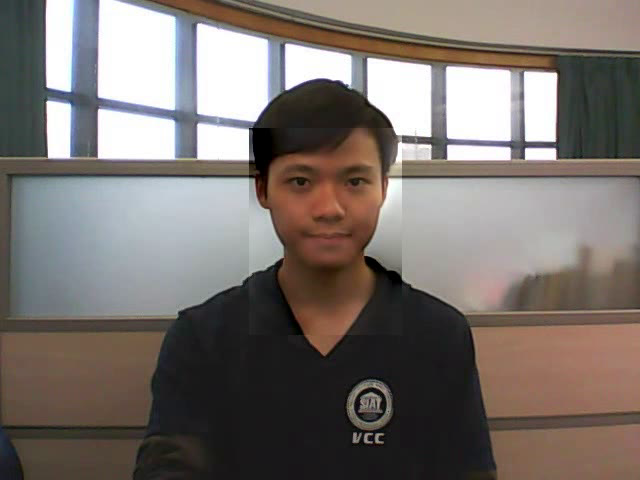
\includegraphics[width=.6\textwidth]{bound-artifact.png}
  \caption{直接对跟踪区域进行动作放大会导致区域边缘出现明显边界}
  \label{fig:bound-artifact}
\end{figure}

为了解决这个问题,本文在进行目标跟踪的同时,使
用GrabCut算法\upcite{Rother2004}从原视频图像帧中提取出目标区域的前景掩码。

GrabCut算法是在Graph Cuts算法的基础上发展而来的一种简单直观的分割算法,其与
Graph Cuts的区别在于:

\begin{compactenum}
\item 混合高斯模型(Gaussian Mixture Model,GMM)。Graph Cut使用灰度直方图作为目
  标和背景的模型,而GrabCut则使用RGB三通道的混合高斯模型。
\item 迭代估计(iterative estimation)。Graph Cuts算法是基于能量最小化一次性完成
  分割的,而GrabCut算法则是一个不断进行分割估计和模型参数学习的迭代过程。
\item 不完全标注(incomplete labelling)。Graph Cuts要求用户在目标和背景中选取一
  些种子点,因而需要较多的交互;而GrabCut只需要用户简单地框选包含目标的区域,就
  足以达到良好的分割效果。
\end{compactenum}

GrabCut的以上几点特性,尤其是不完全标注的特性,使其非常适合用在对目标区域中的前
景区域的进一步分割上:对每帧图像进行区域跟踪所得到的目标区域可以同时作
为GrabCut算法的标注区域。因此,本文的整个算法过程只需用户在参照帧框选一次感兴趣
区域,其他过程都可以自动化进行。

图\ref{fig:grabcut-result}给出了使用GrabCut算法对视频中的某一帧图像进行分割,
提取前景掩码的过程。首先,将该帧的区域跟踪结果作为GrabCut的标注区域进行前景分割,
提取出一幅与原视频帧同样大小的前景掩码。之后,再从该掩码图进一步截取出一幅与目标
区域相同大小的掩码图,这一步是为了在后期将目标区域的动作放大结果与目标区域原图进
行金字塔混合。

\begin{figure}[htbp]
  \centering
  \subfloat[原视频帧]{%
    \label{fig:grabcut-original}
    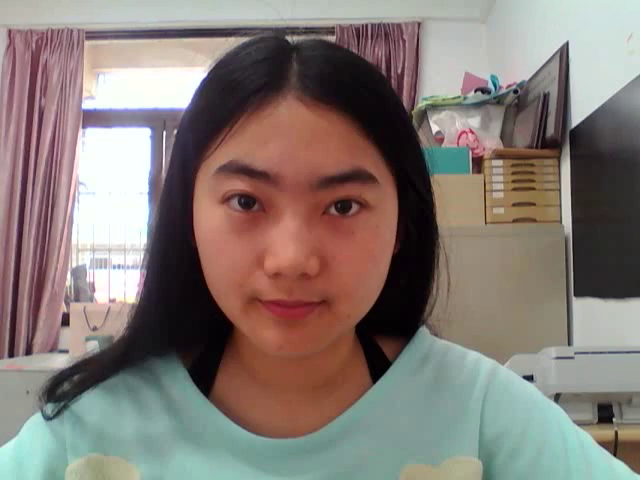
\includegraphics[width=.4\textwidth]{grabcut-original.png}
  }\qquad
  \subfloat[区域跟踪结果]{%
    \label{fig:grabcut-track}
    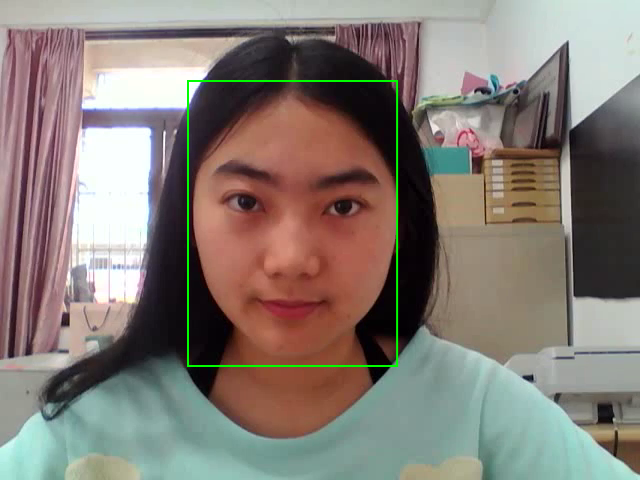
\includegraphics[width=.4\textwidth]{grabcut-track.png}
  }\qquad\\
  \subfloat[使用GrabCut提取得到的前景掩码]{%
    \label{fig:grabcut-mask}
    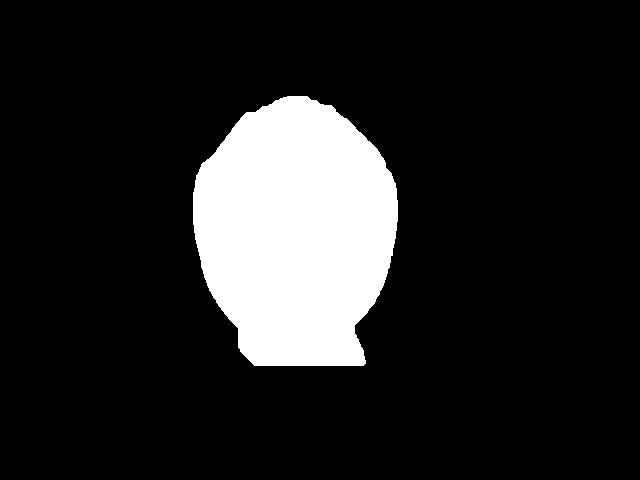
\includegraphics[width=.4\textwidth]{grabcut-mask.png}
  }\qquad
  \subfloat[截取结果]{%
    \label{fig:grabcut-roi}
    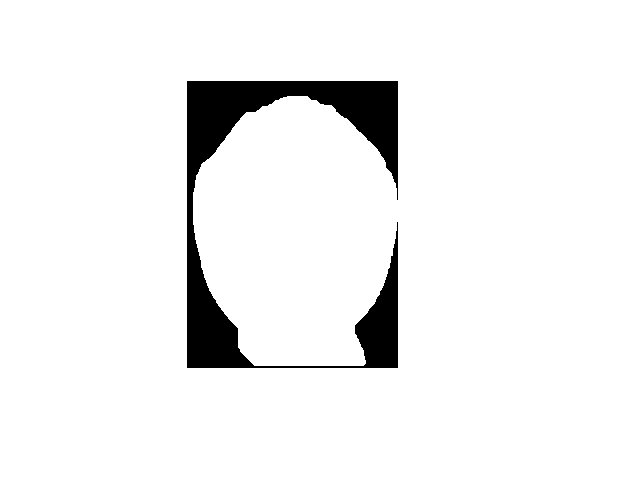
\includegraphics[width=.4\textwidth]{grabcut-roi.png}
  }\qquad
  \caption{使用GrabCut算法从目标区域进一步提取出前景区域}
  \label{fig:grabcut-result}
\end{figure}

\section{局部欧拉影像动作放大}
\label{sec:local-evm}

完成了区域跟踪和前景分割后,接下来对每一帧的目标区域进行欧拉影像动作放大。放大算
法可以使用线性的方法\upcite{wu2012eulerian}或者基于相位的方
法\upcite{Wadhwa2013PhaseBased}。

\subsection{基于CIEL*a*b*空间的颜色衰减}
\label{sec:cielab}

为了抑制噪声,上述两种方法在进行动作放大前,先将视频的每一帧图像由RGB颜色空间转
换为YIQ色彩空间\upcite{buchsbaum1968color}。YIQ是NTSC电视机系统所采用的颜色
空间,其中,Y是亮度信号,I和Q是色相信号。然后分别对Y、I、Q三个通道的进行时
频处理。之后,引入一个衰减因子$\mu$($0\le \mu \le 1$)衰减I、Q两个通道的变化。
如果要放大动作的变化,可以让$\mu$取一个接近0的值,减少对颜色变化的放大,从而
抑制颜色噪点;如果要放大颜色的变化,则可以让$\mu$取一个接近1的值。

与上述方法不同,本文在进行动作放大前,并不将图像从RGB颜色空间转为YIQ色彩空间,
而是转为更感知均匀的CIEL*a*b*颜色空间\upcite{mcguire1992reporting}。其中,L*分
量密切匹配人类亮度感知,a*和b*分量则分别为红/绿和黄/蓝对立通道。L*、a* 和 b*
的非线性关系可以模仿人眼的非线性响应。图\ref{fig:cielab}是CIEL*a*b*颜色空间的
一个彩色模型图。

\begin{figure}[htbp]
  \centering
  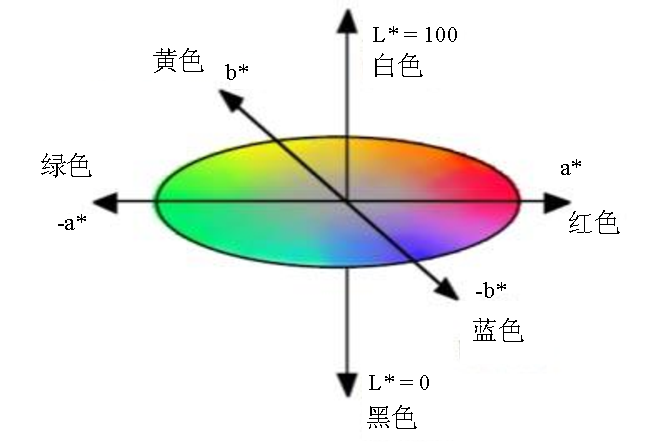
\includegraphics[width=.5\textwidth]{color-plate.pdf}
  \caption{CIEL*a*b*颜色空间模型图}
  \label{fig:cielab}
\end{figure}

要将图像由RGB颜色空间转换到CIEL*a*b*颜色空间,首先先将图像每一个像素的RGB分
量的值归一化为$[0, 1]$之间的浮点数,然后转换到设备无关的XYZ三色值:
\begin{eqnarray*}
  & \begin{bmatrix} X \\ Y \\ Z \end{bmatrix} \leftarrow
  \begin{bmatrix}
    0.412453 & 0.357580 & 0.180423 \\
    0.212671 & 0.715160 & 0.072169 \\
    0.019334 & 0.119193 & 0.950227 \\
  \end{bmatrix}
  \cdot
  \begin{bmatrix}
    R \\ G \\ B
  \end{bmatrix}\\
  & X \leftarrow X/X_n\\
  & Z \leftarrow Z/Z_n
\end{eqnarray*}

其中$X_n = 0.950456$,$Z_n = 1.088754$。

之后将XYZ三色值转为L*、a*、b*的对应值:
\begin{eqnarray*}
  L* & \leftarrow & 116f(Y/Y_n)-16\\
  a* & \leftarrow & 500(f(X/X_n)-f(Y/Y_n))\\
  b* & \leftarrow & 200(f(Y/Y_n)-f(Z/Z_n))
\end{eqnarray*}

其中
\begin{displaymath}
  f(t)=\left\{
    \begin{aligned}
      & t^{1/3} &, t > (\frac{6}{29})^3\\
      & \frac{1}{3}(\frac{29}{6})^2t + \frac{4}{29} &, t \le (\frac{6}{29})^3
    \end{aligned}
\right.
\end{displaymath}

这里的$X_n$,$Y_n$和 $Z_n$是参照白点的CIE XYZ三色值。

将图像由RGB颜色空间转为更加符合人类视觉感知的CIEL*a*b*颜色空间后,对图像进行
动作放大后仍然可以引入衰减因子$\mu$衰减a*、b*两个通道的变化。
图\ref{fig:attenuation}给出了放大face案例的动作后使用$\mu = 0.1$对a*、b*
两个通道的变化进行衰减的结果对比。

\begin{figure}[htbp]
  \centering
  \subfloat[衰减前,图像存在较多颜色噪点]{
    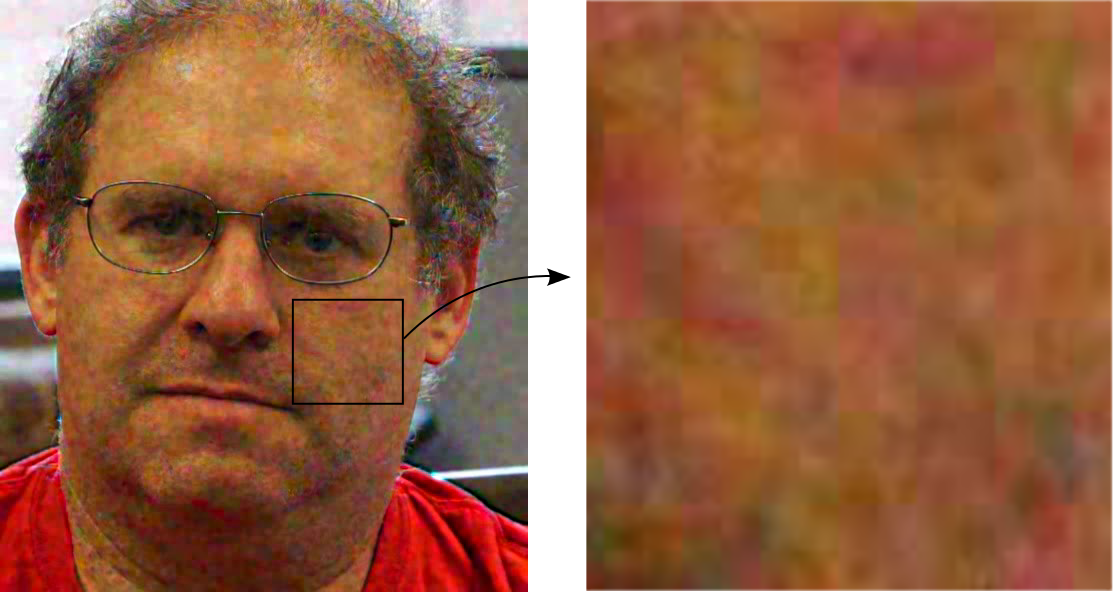
\includegraphics[width=.8\textwidth]{attenuation-before.png}
  }\\
  \subfloat[衰减后,颜色噪点被消除]{
    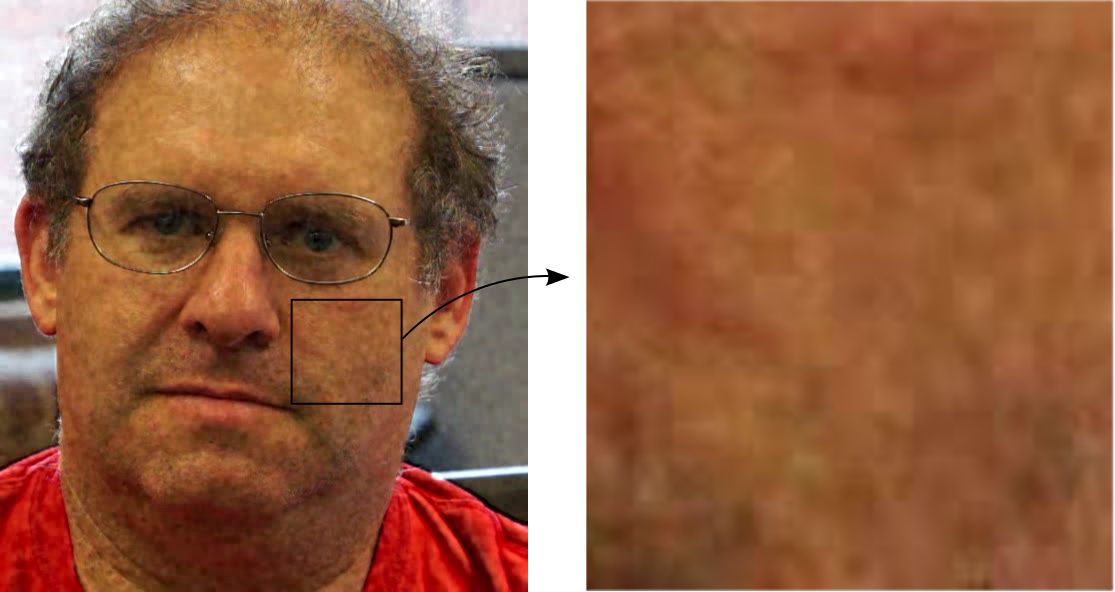
\includegraphics[width=.8\textwidth]{attenuation-after.png}
  }
  \caption{对a*、b*两个通道的变化进行衰减前后结果对比}
  \label{fig:attenuation}
\end{figure}

\subsection{基于四元数的理想带通滤波}
\label{sec:real-quaternion-fourier}

如\ref{sec:eulerian}所述,得到不同空间频率的基带后,对每一基带进行带通滤波,可以
得到感兴趣的变化信号。对于不需要对放大结果进行后续的时频分析的场合,本文使用宽通
带的二阶无限脉冲响应带通滤波器进行带通滤波,该滤波器利用前后帧的差分关系来进行滤
波,因而无需进行时频转换\upcite{storn1996differential};而对于需要对放大结果进行
后续的时频分析的场合,本文使用窄通带的理想带通滤波器进行带通滤波。

对一幅灰度图像进行频率域的理想带通滤波前,需要先对图像进行傅里叶变换,将其转换到
频率域,再构造一个滤波器与之做乘积。二维数字图像的傅里叶变换(DFT)定义为:
\begin{equation}
  \label{eq:dft}
  F(u,v)=\sum_{x=0}^{M-1}\sum_{y=0}^{N-1}f(x,y)e^{-j2\pi(ux/M+vy/N)}
\end{equation}

其中,离散变量$u$,$v$满足$u=0,1,2,\ldots,M-1$,$v=0,1,2,\ldots,N-1$。

由于彩色图像无法直接进行傅里叶变换,因此,文献\cite{wu2012eulerian}及文
献\cite{Wadhwa2013PhaseBased}需要先将每一基带的彩色图像分离成Y、I、Q三个通道图像,
然后对每一个通道的图像单独进行傅里叶变换及带通滤波。

对彩色图像进行理想带通滤波的过程如算
法\ref{alg:temporal-filter}所示\upcite{Gonzalez:2006:DIP:1076432}:

\begin{algorithm}[htbp]
  \caption{理想带通滤波器滤波步骤}
  \label{alg:temporal-filter}
  \begin{algorithmic}[1]
    \REQUIRE 大小为$M\times N$的彩色图像$f(x,y)$。
    \ENSURE 滤波结果$g(x,y)$。
    \STATE 通道分解:将彩色图像$f(x,y)$分成三个通道的图像$f_1(x,y)$,
    $f_2(x,y)$和$f_3(x,y)$。对每幅图像分别执行第2$\sim$7步。
    \STATE 填充图像:对$f_i(x,y)$填充必要数量的0,形成大小为$P\times Q$的填充后的图像
    $f_{p}(x,y)$。其中,$P$和$Q$分别是满足$P\le 2M-1$和$Q\le 2N-1$的最小偶整数。
    \STATE 中心化图像:用$(-1)^{x,y}$乘以$f_{p}(x,y)$,使其移到变换的中心。
    \STATE DFT:根据公式\ref{eq:dft}计算来自步骤3的图像的DFT,得到$F(u,v)$。
    \STATE 理想带通滤波:生成一个实的、对称的理想带通滤波函数 $H(u,v)$,其大小为
    $P\times Q$,中心在$(P/2, Q/2)$处,对图像进行带通滤波操作:$$G(u,v)=H(u,v)F(u,v)$$
    \STATE IDFT:得到处理后的图像:$$g_p(x,y)=\left\{
      \mbox{real}[\Im^{-1}[G(u,v)]] \right\}(-1)^{x+y}$$ 其中,$\Im^{-1}$是IDFT,
    下标$p$用于表明$g_p(x,y)$是填充后的序列。
    \STATE 提取结果:从$g_p(x,y)$的左象限提取$M\times N$区域,得到该通道的滤波结
    果$g_i(x,y)$。
    \STATE 合并通道:将三个单通道的滤波结果$g_1(x,y)$,$g_2(x,y)$和$g_3(x,y)$重新合成一幅彩色图像$g(x,y)$。
  \end{algorithmic}
\end{algorithm}

与上述方法不同,本文在进行理想带通滤波时,并不显式地分离彩色图像的三个通道,而是
将彩色图像的L*、a*、b*三个分量放入一个四元数\upcite{hamilton1866elements}的矢量部
分,形成一个纯四元数。然后直接对其进行傅里叶变换和带通滤波等时频处理,具备更好的整体性。

一个四元数是如下形式的超复数:
\begin{equation}
  \label{eq:quaternion}
  q=a+bi+cj+dk
\end{equation}

其中,$a$、$b$、$c$和$d$是实数,$i$、$j$和$k$是复数单位,且满足:
\begin{equation}
  \label{eq:ijk}
  i^2=j^2=k^2=-1\mbox{,}ij=-ji=k\mbox{,}jk=-kj=i\mbox{,}ik=-ki=-j
\end{equation}

四元数的模定义为:$\left|q\right|=\sqrt{a^2+b^2+c^2+d^2}$,共轭定义为:$\bar{q}=a-bi-cj-dk$。

模为1的四元数称为单位四元数,实部为0的四元数称为纯四元数。

文献\cite{sangwine2000discrete}给出了一般性的四元数傅里叶变换:
\begin{equation}
  \label{eq:quaternion-dft}
  F(u,v)=\frac{1}{\sqrt{MN}}\sum_{y=0}^{M-1}\sum_{x=0}^{N-1}e^{-\mu 2\pi((yv/M)+(xu/N))}f(x,y)
\end{equation}

在本文中,$f$是包含了L*,a*,b*三个分量的二维向量,即
\begin{equation}
  \label{eq:quaternion-lab}
  f(x,y)=L^{*}(x,y)i+a^{*}(x,y)j+b^{*}(x,y)k
\end{equation}

算法\ref{alg:quaternion-temporal-filter}给出了基于四元数的理想带通滤波的步骤。

\begin{algorithm}[htbp]
  \caption{基于四元数的理想带通滤波器滤波步骤}
  \label{alg:quaternion-temporal-filter}
  \begin{algorithmic}[1]
    \REQUIRE 大小为$M\times N$的四元数向量$f(x,y)$。
    \ENSURE 滤波结果 $g(x,y)$。
    \STATE 填充图像:对$f(x,y)$填充必要数量的0,形成大小为$P\times Q$的填充后的图像
    $f_{p}(x,y)$。其中,$P$和$Q$分别是满足$P\le 2M-1$和$Q\le 2N-1$的最小偶整数。
    \STATE 中心化图像:用$(-1)^{x,y}$乘以$f_{p}(x,y)$,使其移到变换的中心。
    \STATE DFT:根据公式\ref{eq:quaternion-dft}计算来自步骤3的图像的DFT,得到$F(u,v)$。
    \STATE 理想带通滤波:生成一个实的、对称的理想带通滤波函数 $H(u,v)$,其大小为
    $P\times Q$,中心在$(P/2, Q/2)$处,对图像进行带通滤波操作:$$G(u,v)=H(u,v)F(u,v)$$
    \STATE IDFT:得到处理后的图像:$$g_p(x,y)=\left\{
      \mbox{real}[\Im^{-1}[G(u,v)]] \right\}(-1)^{x+y}$$ 其中,$\Im^{-1}$是IDFT,
    下标$p$用于表明$g_p(x,y)$是填充后的序列。
    \STATE 提取结果:从$g_p(x,y)$的左象限提取$M\times N$区域,得到该通道的滤波结
    果$g(x,y)$。
  \end{algorithmic}
\end{algorithm}


\section{金字塔混合}
\label{sec:pyramid-blending}

如第\ref{sec:grabcut}节所述,直接对目标区域组成的图像序列进行动作放大会把背景
部分的动作也一同放大。因此,可利用每一帧目标区域对应的前景掩码,将放大结果进一步
约束在前景区域。

最直接的做法是单基带混合:利用前景掩码,从经过放大的动作中取出前景的部分,然后与
原图叠加。但由于动作信号被放大后,部分像素的亮度会增加,此时如果直接与原图叠加,
在目标区域与其他区域间仍然可能出现较生硬的边界。因此,本文采用多基带的金字塔混合
的方法\upcite{ogden1985pyramid},利用前景掩码对目标区域原图和动作放大结果进行金字
塔混合。

考虑图像$A$ 、图像$B$以及掩码图$M$。则对$A$和$B$进行金字塔混合的步骤如算
法\ref{alg:blend}所示。

\begin{algorithm}[htbp]
  \caption{金字塔混合}
  \label{alg:blend}
  \begin{algorithmic}[1]
    \REQUIRE 大小相同的图像$A$,图像$B$及掩码图$M$。
    \ENSURE 混合结果$C$。
    \STATE 分别由图像$A$和图像$B$构造$n$层拉普拉斯金字塔$P_A$和$P_B$,
    由图像$M$构造$n$层高斯金字塔$P_M$。
    \STATE 对每一层基带,单独进行上述的单基带混合,将混合结果存入一个新的拉普拉
    斯金字塔$P_C$的相同层。
    \STATE 根据$P_C$重建出图像$C$ 。
  \end{algorithmic}
\end{algorithm}

在本文中,$P_A$、$P_B$分别是经放大后的动作信息和原图的拉普拉斯金字塔,而$P_M$则
为前景掩码的高斯金字塔,这三个图像金字塔在进行欧拉影像动作放大时已经构造完成,因
此无需再执行算法\ref{alg:blend}中的第1步。

图\ref{fig:blend-compare}给出了单基带混合和金字塔混合的结果对比。经过单基带混合
后,女孩的脖子处依然存在明显的边界。而经过金字塔混合后,脖子处的边界已经被消除。

\clearpage

\begin{figure}[htbp]
  \centering
  \subfloat[单基带混合,仍然可能存在边界]{
    \label{fig:single-band}
  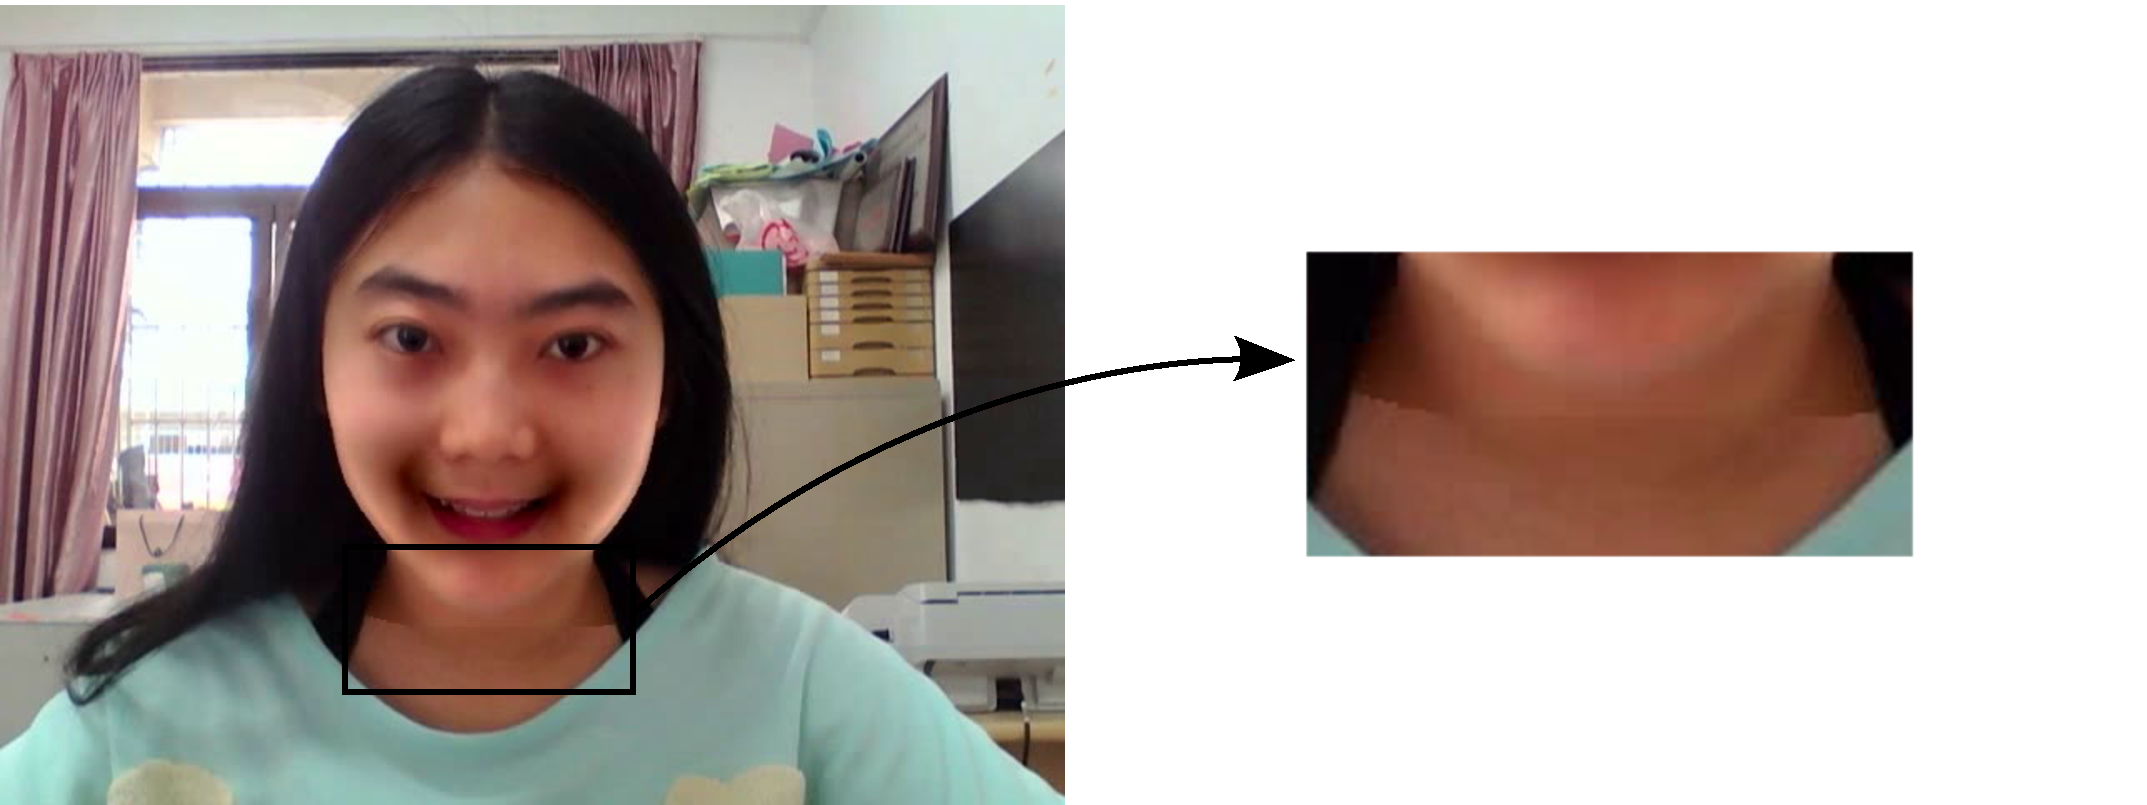
\includegraphics[width=.8\textwidth]{single-band-blend-asy.pdf}
  }\\
  \subfloat[金字塔混合,边界问题得到改善]{
    \label{fig:multi-band}
    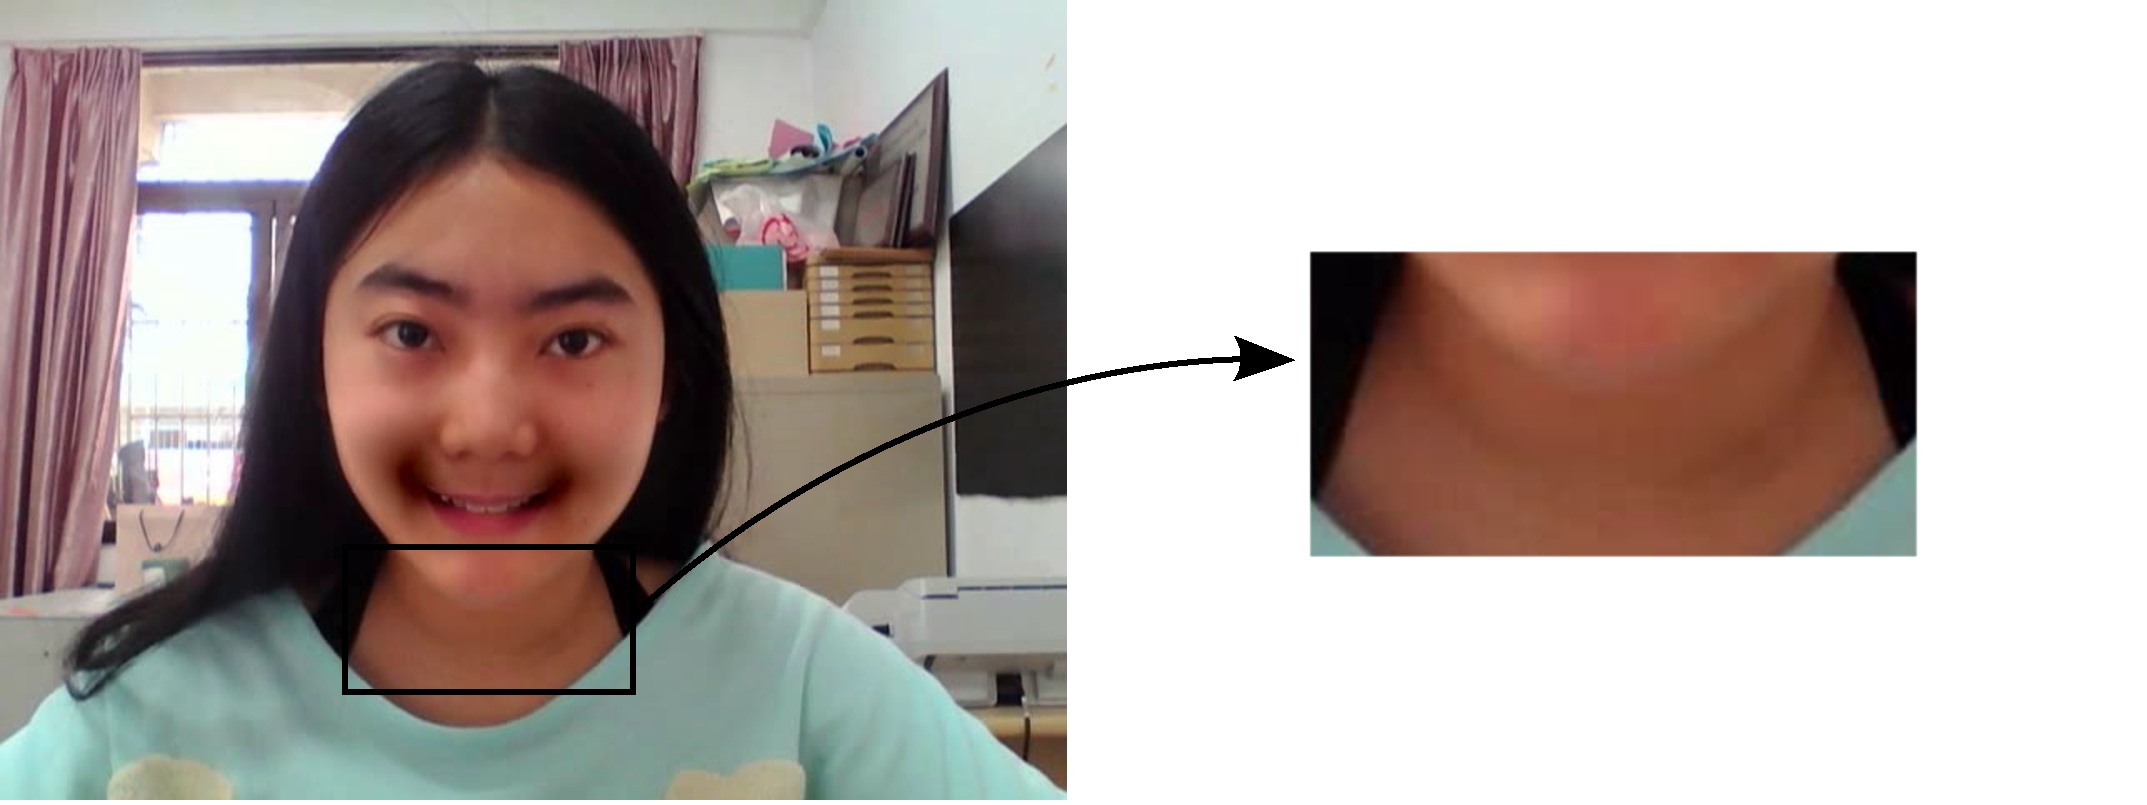
\includegraphics[width=.8\textwidth]{pyramid-blend-asy.pdf}
  }
  \caption{单基带混合和金字塔混合的结果对比}
  \label{fig:blend-compare}
\end{figure}

%%% Local Variables: 
%%% mode: latex
%%% TeX-master: "../thesis"
%%% End: 

